% REV00 Tue 04 May 2021 13:55:16 WIB
% START Tue 04 May 2021 13:55:16 WIB

\chapter{XXX}

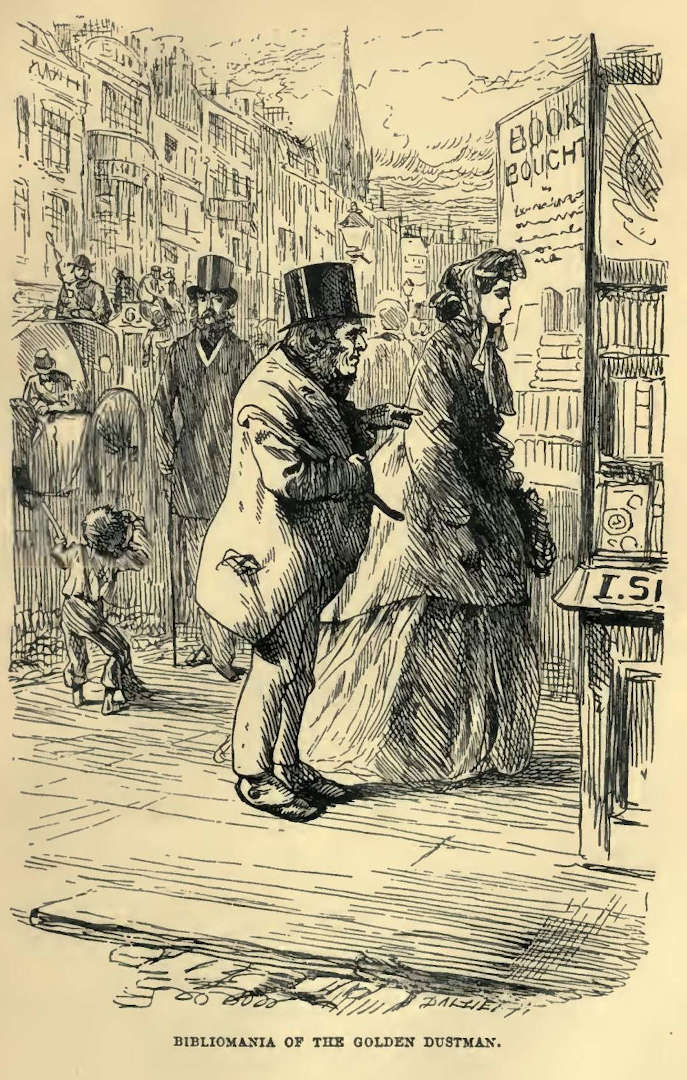
\includegraphics[scale=2.3]{03-05-01}

Chapter 17

THE VOICE OF SOCIETY


Behoves Mortimer Lightwood, therefore, to answer a dinner card from Mr
and Mrs Veneering requesting the honour, and to signify that Mr Mortimer
Lightwood will be happy to have the other honour. The Veneerings have
been, as usual, indefatigably dealing dinner cards to Society, and
whoever desires to take a hand had best be quick about it, for it is
written in the Books of the Insolvent Fates that Veneering shall make a
resounding smash next week. Yes. Having found out the clue to that great
mystery how people can contrive to live beyond their means, and having
over-jobbed his jobberies as legislator deputed to the Universe by the
pure electors of Pocket-Breaches, it shall come to pass next week that
Veneering will accept the Chiltern Hundreds, that the legal gentleman in
Britannia’s confidence will again accept the Pocket-Breaches Thousands,
and that the Veneerings will retire to Calais, there to live on Mrs
Veneering’s diamonds (in which Mr Veneering, as a good husband, has from
time to time invested considerable sums), and to relate to Neptune and
others, how that, before Veneering retired from Parliament, the House
of Commons was composed of himself and the six hundred and fifty-seven
dearest and oldest friends he had in the world. It shall likewise come
to pass, at as nearly as possible the same period, that Society will
discover that it always did despise Veneering, and distrust Veneering,
and that when it went to Veneering’s to dinner it always had
misgivings--though very secretly at the time, it would seem, and in a
perfectly private and confidential manner.

The next week’s books of the Insolvent Fates, however, being not yet
opened, there is the usual rush to the Veneerings, of the people who go
to their house to dine with one another and not with them. There is Lady
Tippins. There are Podsnap the Great, and Mrs Podsnap. There is Twemlow.
There are Buffer, Boots, and Brewer. There is the Contractor, who
is Providence to five hundred thousand men. There is the Chairman,
travelling three thousand miles per week. There is the brilliant genius
who turned the shares into that remarkably exact sum of three hundred
and seventy five thousand pounds, no shillings, and nopence.

To whom, add Mortimer Lightwood, coming in among them with a
reassumption of his old languid air, founded on Eugene, and belonging to
the days when he told the story of the man from Somewhere.

That fresh fairy, Tippins, all but screams at sight of her false
swain. She summons the deserter to her with her fan; but the deserter,
predetermined not to come, talks Britain with Podsnap. Podsnap always
talks Britain, and talks as if he were a sort of Private Watchman
employed, in the British interests, against the rest of the world. ‘We
know what Russia means, sir,’ says Podsnap; ‘we know what France wants;
we see what America is up to; but we know what England is. That’s enough
for us.’

However, when dinner is served, and Lightwood drops into his old place
over against Lady Tippins, she can be fended off no longer. ‘Long
banished Robinson Crusoe,’ says the charmer, exchanging salutations,
‘how did you leave the Island?’

‘Thank you,’ says Lightwood. ‘It made no complaint of being in pain
anywhere.’

‘Say, how did you leave the savages?’ asks Lady Tippins.

‘They were becoming civilized when I left Juan Fernandez,’ says
Lightwood. ‘At least they were eating one another, which looked like
it.’

‘Tormentor!’ returns the dear young creature. ‘You know what I mean, and
you trifle with my impatience. Tell me something, immediately, about the
married pair. You were at the wedding.’

‘Was I, by-the-by?’ Mortimer pretends, at great leisure, to consider.
‘So I was!’

‘How was the bride dressed? In rowing costume?’

Mortimer looks gloomy, and declines to answer.

‘I hope she steered herself, skiffed herself, paddled herself,
larboarded and starboarded herself, or whatever the technical term may
be, to the ceremony?’ proceeds the playful Tippins.

‘However she got to it, she graced it,’ says Mortimer.

Lady Tippins with a skittish little scream, attracts the general
attention. ‘Graced it! Take care of me if I faint, Veneering. He means
to tell us, that a horrid female waterman is graceful!’

‘Pardon me. I mean to tell you nothing, Lady Tippins,’ replies
Lightwood. And keeps his word by eating his dinner with a show of the
utmost indifference.

‘You shall not escape me in this way, you morose backwoodsman,’ retorts
Lady Tippins. ‘You shall not evade the question, to screen your friend
Eugene, who has made this exhibition of himself. The knowledge shall be
brought home to you that such a ridiculous affair is condemned by the
voice of Society. My dear Mrs Veneering, do let us resolve ourselves
into a Committee of the whole House on the subject.’

Mrs Veneering, always charmed by this rattling sylph, cries. ‘Oh yes!
Do let us resolve ourselves into a Committee of the whole House!
So delicious!’ Veneering says, ‘As many as are of that opinion, say
Aye,--contrary, No--the Ayes have it.’ But nobody takes the slightest
notice of his joke.

‘Now, I am Chairwoman of Committees!’ cries Lady Tippins.

[‘What spirits she has!’ exclaims Mrs Veneering; to whom likewise nobody
attends.)

‘And this,’ pursues the sprightly one, ‘is a Committee of the whole
House to what-you-may-call-it--elicit, I suppose--the voice of Society.
The question before the Committee is, whether a young man of very fair
family, good appearance, and some talent, makes a fool or a wise man of
himself in marrying a female waterman, turned factory girl.’

‘Hardly so, I think,’ the stubborn Mortimer strikes in. ‘I take the
question to be, whether such a man as you describe, Lady Tippins, does
right or wrong in marrying a brave woman (I say nothing of her beauty),
who has saved his life, with a wonderful energy and address; whom he
knows to be virtuous, and possessed of remarkable qualities; whom he has
long admired, and who is deeply attached to him.’

‘But, excuse me,’ says Podsnap, with his temper and his shirt-collar
about equally rumpled; ‘was this young woman ever a female waterman?’

‘Never. But she sometimes rowed in a boat with her father, I believe.’

General sensation against the young woman. Brewer shakes his head. Boots
shakes his head. Buffer shakes his head.

‘And now, Mr Lightwood, was she ever,’ pursues Podsnap, with his
indignation rising high into those hair-brushes of his, ‘a factory
girl?’

‘Never. But she had some employment in a paper mill, I believe.’

General sensation repeated. Brewer says, ‘Oh dear!’ Boots says, ‘Oh
dear!’ Buffer says, ‘Oh dear!’ All, in a rumbling tone of protest.

‘Then all I have to say is,’ returns Podsnap, putting the thing away
with his right arm, ‘that my gorge rises against such a marriage--that
it offends and disgusts me--that it makes me sick--and that I desire to
know no more about it.’

[‘Now I wonder,’ thinks Mortimer, amused, ‘whether YOU are the Voice of
Society!’)

‘Hear, hear, hear!’ cries Lady Tippins. ‘Your opinion of this
MESALLIANCE, honourable colleagues of the honourable member who has just
sat down?’

Mrs Podsnap is of opinion that in these matters there should be an
equality of station and fortune, and that a man accustomed to Society
should look out for a woman accustomed to Society and capable of bearing
her part in it with--an ease and elegance of carriage--that.’ Mrs
Podsnap stops there, delicately intimating that every such man should
look out for a fine woman as nearly resembling herself as he may hope to
discover.

[‘Now I wonder,’ thinks Mortimer, ‘whether you are the Voice!’)

Lady Tippins next canvasses the Contractor, of five hundred thousand
power. It appears to this potentate, that what the man in question
should have done, would have been, to buy the young woman a boat and a
small annuity, and set her up for herself. These things are a question
of beefsteaks and porter. You buy the young woman a boat. Very good. You
buy her, at the same time, a small annuity. You speak of that annuity in
pounds sterling, but it is in reality so many pounds of beefsteaks and
so many pints of porter. On the one hand, the young woman has the boat.
On the other hand, she consumes so many pounds of beefsteaks and so many
pints of porter. Those beefsteaks and that porter are the fuel to that
young woman’s engine. She derives therefrom a certain amount of power to
row the boat; that power will produce so much money; you add that to the
small annuity; and thus you get at the young woman’s income. That (it
seems to the Contractor) is the way of looking at it.

The fair enslaver having fallen into one of her gentle sleeps during the
last exposition, nobody likes to wake her. Fortunately, she comes
awake of herself, and puts the question to the Wandering Chairman. The
Wanderer can only speak of the case as if it were his own. If such a
young woman as the young woman described, had saved his own life, he
would have been very much obliged to her, wouldn’t have married her, and
would have got her a berth in an Electric Telegraph Office, where young
women answer very well.

What does the Genius of the three hundred and seventy-five thousand
pounds, no shillings, and nopence, think? He can’t say what he thinks,
without asking: Had the young woman any money?

‘No,’ says Lightwood, in an uncompromising voice; ‘no money.’

‘Madness and moonshine,’ is then the compressed verdict of the Genius.
‘A man may do anything lawful, for money. But for no money!--Bosh!’

What does Boots say?

Boots says he wouldn’t have done it under twenty thousand pound.

What does Brewer say?

Brewer says what Boots says.

What does Buffer say?

Buffer says he knows a man who married a bathing-woman, and bolted.

Lady Tippins fancies she has collected the suffrages of the whole
Committee (nobody dreaming of asking the Veneerings for their opinion),
when, looking round the table through her eyeglass, she perceives Mr
Twemlow with his hand to his forehead.

Good gracious! My Twemlow forgotten! My dearest! My own! What is his
vote?

Twemlow has the air of being ill at ease, as he takes his hand from his
forehead and replies.

‘I am disposed to think,’ says he, ‘that this is a question of the
feelings of a gentleman.’

‘A gentleman can have no feelings who contracts such a marriage,’
flushes Podsnap.

‘Pardon me, sir,’ says Twemlow, rather less mildly than usual, ‘I don’t
agree with you. If this gentleman’s feelings of gratitude, of respect,
of admiration, and affection, induced him (as I presume they did) to
marry this lady--’

‘This lady!’ echoes Podsnap.

‘Sir,’ returns Twemlow, with his wristbands bristling a little, ‘YOU
repeat the word; I repeat the word. This lady. What else would you call
her, if the gentleman were present?’

This being something in the nature of a poser for Podsnap, he merely
waves it away with a speechless wave.

‘I say,’ resumes Twemlow, ‘if such feelings on the part of this
gentleman, induced this gentleman to marry this lady, I think he is the
greater gentleman for the action, and makes her the greater lady. I beg
to say, that when I use the word, gentleman, I use it in the sense in
which the degree may be attained by any man. The feelings of a gentleman
I hold sacred, and I confess I am not comfortable when they are made the
subject of sport or general discussion.’

‘I should like to know,’ sneers Podsnap, ‘whether your noble relation
would be of your opinion.’

‘Mr Podsnap,’ retorts Twemlow, ‘permit me. He might be, or he might not
be. I cannot say. But, I could not allow even him to dictate to me on a
point of great delicacy, on which I feel very strongly.’

Somehow, a canopy of wet blanket seems to descend upon the company, and
Lady Tippins was never known to turn so very greedy or so very cross.
Mortimer Lightwood alone brightens. He has been asking himself, as to
every other member of the Committee in turn, ‘I wonder whether you are
the Voice!’ But he does not ask himself the question after Twemlow has
spoken, and he glances in Twemlow’s direction as if he were grateful.
When the company disperse--by which time Mr and Mrs Veneering have had
quite as much as they want of the honour, and the guests have had quite
as much as THEY want of the other honour--Mortimer sees Twemlow home,
shakes hands with him cordially at parting, and fares to the Temple,
gaily.



POSTSCRIPT

IN LIEU OF PREFACE


When I devised this story, I foresaw the likelihood that a class of
readers and commentators would suppose that I was at great pains to
conceal exactly what I was at great pains to suggest: namely, that Mr
John Harmon was not slain, and that Mr John Rokesmith was he. Pleasing
myself with the idea that the supposition might in part arise out
of some ingenuity in the story, and thinking it worth while, in the
interests of art, to hint to an audience that an artist (of whatever
denomination) may perhaps be trusted to know what he is about in his
vocation, if they will concede him a little patience, I was not alarmed
by the anticipation.

To keep for a long time unsuspected, yet always working itself out,
another purpose originating in that leading incident, and turning it to
a pleasant and useful account at last, was at once the most interesting
and the most difficult part of my design. Its difficulty was much
enhanced by the mode of publication; for, it would be very unreasonable
to expect that many readers, pursuing a story in portions from month
to month through nineteen months, will, until they have it before them
complete, perceive the relations of its finer threads to the whole
pattern which is always before the eyes of the story-weaver at his loom.
Yet, that I hold the advantages of the mode of publication to outweigh
its disadvantages, may be easily believed of one who revived it in the
Pickwick Papers after long disuse, and has pursued it ever since.

There is sometimes an odd disposition in this country to dispute as
improbable in fiction, what are the commonest experiences in fact.
Therefore, I note here, though it may not be at all necessary, that
there are hundreds of Will Cases (as they are called), far more
remarkable than that fancied in this book; and that the stores of the
Prerogative Office teem with instances of testators who have made,
changed, contradicted, hidden, forgotten, left cancelled, and left
uncancelled, each many more wills than were ever made by the elder Mr
Harmon of Harmony Jail.

In my social experiences since Mrs Betty Higden came upon the scene and
left it, I have found Circumlocutional champions disposed to be
warm with me on the subject of my view of the Poor Law. Mr friend Mr
Bounderby could never see any difference between leaving the Coketown
‘hands’ exactly as they were, and requiring them to be fed with turtle
soup and venison out of gold spoons. Idiotic propositions of a parallel
nature have been freely offered for my acceptance, and I have been
called upon to admit that I would give Poor Law relief to anybody,
anywhere, anyhow. Putting this nonsense aside, I have observed a
suspicious tendency in the champions to divide into two parties; the
one, contending that there are no deserving Poor who prefer death by
slow starvation and bitter weather, to the mercies of some Relieving
Officers and some Union Houses; the other, admitting that there are such
Poor, but denying that they have any cause or reason for what they do.
The records in our newspapers, the late exposure by THE LANCET, and the
common sense and senses of common people, furnish too abundant evidence
against both defences. But, that my view of the Poor Law may not be
mistaken or misrepresented, I will state it. I believe there has been
in England, since the days of the STUARTS, no law so often infamously
administered, no law so often openly violated, no law habitually so
ill-supervised. In the majority of the shameful cases of disease and
death from destitution, that shock the Public and disgrace the country,
the illegality is quite equal to the inhumanity--and known language
could say no more of their lawlessness.

On Friday the Ninth of June in the present year, Mr and Mrs Boffin (in
their manuscript dress of receiving Mr and Mrs Lammle at breakfast)
were on the South Eastern Railway with me, in a terribly destructive
accident. When I had done what I could to help others, I climbed back
into my carriage--nearly turned over a viaduct, and caught aslant upon
the turn--to extricate the worthy couple. They were much soiled, but
otherwise unhurt. The same happy result attended Miss Bella Wilfer on
her wedding day, and Mr Riderhood inspecting Bradley Headstone’s red
neckerchief as he lay asleep. I remember with devout thankfulness that I
can never be much nearer parting company with my readers for ever, than
I was then, until there shall be written against my life, the two words
with which I have this day closed this book:--THE END.

September 2nd, 1865.





End of the Project Gutenberg EBook of Our Mutual Friend, by Charles Dickens

*** END OF THIS PROJECT GUTENBERG EBOOK OUR MUTUAL FRIEND ***

***** This file should be named 883-0.txt or 883-0.zip *****
This and all associated files of various formats will be found in:
        http://www.gutenberg.org/8/8/883/

Produced by Donald Lainson; David Widger

Updated editions will replace the previous one--the old editions
will be renamed.

Creating the works from public domain print editions means that no
one owns a United States copyright in these works, so the Foundation
(and you!) can copy and distribute it in the United States without
permission and without paying copyright royalties.  Special rules,
set forth in the General Terms of Use part of this license, apply to
copying and distributing Project Gutenberg-tm electronic works to
protect the PROJECT GUTENBERG-tm concept and trademark.  Project
Gutenberg is a registered trademark, and may not be used if you
charge for the eBooks, unless you receive specific permission.  If you
do not charge anything for copies of this eBook, complying with the
rules is very easy.  You may use this eBook for nearly any purpose
such as creation of derivative works, reports, performances and
research.  They may be modified and printed and given away--you may do
practically ANYTHING with public domain eBooks.  Redistribution is
subject to the trademark license, especially commercial
redistribution.



*** START: FULL LICENSE ***

THE FULL PROJECT GUTENBERG LICENSE
PLEASE READ THIS BEFORE YOU DISTRIBUTE OR USE THIS WORK

To protect the Project Gutenberg-tm mission of promoting the free
distribution of electronic works, by using or distributing this work
(or any other work associated in any way with the phrase “Project
Gutenberg”), you agree to comply with all the terms of the Full Project
Gutenberg-tm License (available with this file or online at
http://gutenberg.org/license).


Section 1.  General Terms of Use and Redistributing Project Gutenberg-tm
electronic works

1.A.  By reading or using any part of this Project Gutenberg-tm
electronic work, you indicate that you have read, understand, agree to
and accept all the terms of this license and intellectual property
(trademark/copyright) agreement.  If you do not agree to abide by all
the terms of this agreement, you must cease using and return or destroy
all copies of Project Gutenberg-tm electronic works in your possession.
If you paid a fee for obtaining a copy of or access to a Project
Gutenberg-tm electronic work and you do not agree to be bound by the
terms of this agreement, you may obtain a refund from the person or
entity to whom you paid the fee as set forth in paragraph 1.E.8.

1.B.  “Project Gutenberg” is a registered trademark.  It may only be
used on or associated in any way with an electronic work by people who
agree to be bound by the terms of this agreement.  There are a few
things that you can do with most Project Gutenberg-tm electronic works
even without complying with the full terms of this agreement.  See
paragraph 1.C below.  There are a lot of things you can do with Project
Gutenberg-tm electronic works if you follow the terms of this agreement
and help preserve free future access to Project Gutenberg-tm electronic
works.  See paragraph 1.E below.

1.C.  The Project Gutenberg Literary Archive Foundation (“the Foundation”
 or PGLAF), owns a compilation copyright in the collection of Project
Gutenberg-tm electronic works.  Nearly all the individual works in the
collection are in the public domain in the United States.  If an
individual work is in the public domain in the United States and you are
located in the United States, we do not claim a right to prevent you from
copying, distributing, performing, displaying or creating derivative
works based on the work as long as all references to Project Gutenberg
are removed.  Of course, we hope that you will support the Project
Gutenberg-tm mission of promoting free access to electronic works by
freely sharing Project Gutenberg-tm works in compliance with the terms of
this agreement for keeping the Project Gutenberg-tm name associated with
the work.  You can easily comply with the terms of this agreement by
keeping this work in the same format with its attached full Project
Gutenberg-tm License when you share it without charge with others.

1.D.  The copyright laws of the place where you are located also govern
what you can do with this work.  Copyright laws in most countries are in
a constant state of change.  If you are outside the United States, check
the laws of your country in addition to the terms of this agreement
before downloading, copying, displaying, performing, distributing or
creating derivative works based on this work or any other Project
Gutenberg-tm work.  The Foundation makes no representations concerning
the copyright status of any work in any country outside the United
States.

1.E.  Unless you have removed all references to Project Gutenberg:

1.E.1.  The following sentence, with active links to, or other immediate
access to, the full Project Gutenberg-tm License must appear prominently
whenever any copy of a Project Gutenberg-tm work (any work on which the
phrase “Project Gutenberg” appears, or with which the phrase “Project
Gutenberg” is associated) is accessed, displayed, performed, viewed,
copied or distributed:

This eBook is for the use of anyone anywhere at no cost and with
almost no restrictions whatsoever.  You may copy it, give it away or
re-use it under the terms of the Project Gutenberg License included
with this eBook or online at www.gutenberg.org

1.E.2.  If an individual Project Gutenberg-tm electronic work is derived
from the public domain (does not contain a notice indicating that it is
posted with permission of the copyright holder), the work can be copied
and distributed to anyone in the United States without paying any fees
or charges.  If you are redistributing or providing access to a work
with the phrase “Project Gutenberg” associated with or appearing on the
work, you must comply either with the requirements of paragraphs 1.E.1
through 1.E.7 or obtain permission for the use of the work and the
Project Gutenberg-tm trademark as set forth in paragraphs 1.E.8 or
1.E.9.

1.E.3.  If an individual Project Gutenberg-tm electronic work is posted
with the permission of the copyright holder, your use and distribution
must comply with both paragraphs 1.E.1 through 1.E.7 and any additional
terms imposed by the copyright holder.  Additional terms will be linked
to the Project Gutenberg-tm License for all works posted with the
permission of the copyright holder found at the beginning of this work.

1.E.4.  Do not unlink or detach or remove the full Project Gutenberg-tm
License terms from this work, or any files containing a part of this
work or any other work associated with Project Gutenberg-tm.

1.E.5.  Do not copy, display, perform, distribute or redistribute this
electronic work, or any part of this electronic work, without
prominently displaying the sentence set forth in paragraph 1.E.1 with
active links or immediate access to the full terms of the Project
Gutenberg-tm License.

1.E.6.  You may convert to and distribute this work in any binary,
compressed, marked up, nonproprietary or proprietary form, including any
word processing or hypertext form.  However, if you provide access to or
distribute copies of a Project Gutenberg-tm work in a format other than
“Plain Vanilla ASCII” or other format used in the official version
posted on the official Project Gutenberg-tm web site (www.gutenberg.org),
you must, at no additional cost, fee or expense to the user, provide a
copy, a means of exporting a copy, or a means of obtaining a copy upon
request, of the work in its original “Plain Vanilla ASCII” or other
form.  Any alternate format must include the full Project Gutenberg-tm
License as specified in paragraph 1.E.1.

1.E.7.  Do not charge a fee for access to, viewing, displaying,
performing, copying or distributing any Project Gutenberg-tm works
unless you comply with paragraph 1.E.8 or 1.E.9.

1.E.8.  You may charge a reasonable fee for copies of or providing
access to or distributing Project Gutenberg-tm electronic works provided
that

- You pay a royalty fee of 20% of the gross profits you derive from
     the use of Project Gutenberg-tm works calculated using the method
     you already use to calculate your applicable taxes.  The fee is
     owed to the owner of the Project Gutenberg-tm trademark, but he
     has agreed to donate royalties under this paragraph to the
     Project Gutenberg Literary Archive Foundation.  Royalty payments
     must be paid within 60 days following each date on which you
     prepare (or are legally required to prepare) your periodic tax
     returns.  Royalty payments should be clearly marked as such and
     sent to the Project Gutenberg Literary Archive Foundation at the
     address specified in Section 4, “Information about donations to
     the Project Gutenberg Literary Archive Foundation.”

- You provide a full refund of any money paid by a user who notifies
     you in writing (or by e-mail) within 30 days of receipt that s/he
     does not agree to the terms of the full Project Gutenberg-tm
     License.  You must require such a user to return or
     destroy all copies of the works possessed in a physical medium
     and discontinue all use of and all access to other copies of
     Project Gutenberg-tm works.

- You provide, in accordance with paragraph 1.F.3, a full refund of any
     money paid for a work or a replacement copy, if a defect in the
     electronic work is discovered and reported to you within 90 days
     of receipt of the work.

- You comply with all other terms of this agreement for free
     distribution of Project Gutenberg-tm works.

1.E.9.  If you wish to charge a fee or distribute a Project Gutenberg-tm
electronic work or group of works on different terms than are set
forth in this agreement, you must obtain permission in writing from
both the Project Gutenberg Literary Archive Foundation and Michael
Hart, the owner of the Project Gutenberg-tm trademark.  Contact the
Foundation as set forth in Section 3 below.

1.F.

1.F.1.  Project Gutenberg volunteers and employees expend considerable
effort to identify, do copyright research on, transcribe and proofread
public domain works in creating the Project Gutenberg-tm
collection.  Despite these efforts, Project Gutenberg-tm electronic
works, and the medium on which they may be stored, may contain
“Defects,” such as, but not limited to, incomplete, inaccurate or
corrupt data, transcription errors, a copyright or other intellectual
property infringement, a defective or damaged disk or other medium, a
computer virus, or computer codes that damage or cannot be read by
your equipment.

1.F.2.  LIMITED WARRANTY, DISCLAIMER OF DAMAGES - Except for the “Right
of Replacement or Refund” described in paragraph 1.F.3, the Project
Gutenberg Literary Archive Foundation, the owner of the Project
Gutenberg-tm trademark, and any other party distributing a Project
Gutenberg-tm electronic work under this agreement, disclaim all
liability to you for damages, costs and expenses, including legal
fees.  YOU AGREE THAT YOU HAVE NO REMEDIES FOR NEGLIGENCE, STRICT
LIABILITY, BREACH OF WARRANTY OR BREACH OF CONTRACT EXCEPT THOSE
PROVIDED IN PARAGRAPH F3.  YOU AGREE THAT THE FOUNDATION, THE
TRADEMARK OWNER, AND ANY DISTRIBUTOR UNDER THIS AGREEMENT WILL NOT BE
LIABLE TO YOU FOR ACTUAL, DIRECT, INDIRECT, CONSEQUENTIAL, PUNITIVE OR
INCIDENTAL DAMAGES EVEN IF YOU GIVE NOTICE OF THE POSSIBILITY OF SUCH
DAMAGE.

1.F.3.  LIMITED RIGHT OF REPLACEMENT OR REFUND - If you discover a
defect in this electronic work within 90 days of receiving it, you can
receive a refund of the money (if any) you paid for it by sending a
written explanation to the person you received the work from.  If you
received the work on a physical medium, you must return the medium with
your written explanation.  The person or entity that provided you with
the defective work may elect to provide a replacement copy in lieu of a
refund.  If you received the work electronically, the person or entity
providing it to you may choose to give you a second opportunity to
receive the work electronically in lieu of a refund.  If the second copy
is also defective, you may demand a refund in writing without further
opportunities to fix the problem.

1.F.4.  Except for the limited right of replacement or refund set forth
in paragraph 1.F.3, this work is provided to you ‘AS-IS’ WITH NO OTHER
WARRANTIES OF ANY KIND, EXPRESS OR IMPLIED, INCLUDING BUT NOT LIMITED TO
WARRANTIES OF MERCHANTIBILITY OR FITNESS FOR ANY PURPOSE.

1.F.5.  Some states do not allow disclaimers of certain implied
warranties or the exclusion or limitation of certain types of damages.
If any disclaimer or limitation set forth in this agreement violates the
law of the state applicable to this agreement, the agreement shall be
interpreted to make the maximum disclaimer or limitation permitted by
the applicable state law.  The invalidity or unenforceability of any
provision of this agreement shall not void the remaining provisions.

1.F.6.  INDEMNITY - You agree to indemnify and hold the Foundation, the
trademark owner, any agent or employee of the Foundation, anyone
providing copies of Project Gutenberg-tm electronic works in accordance
with this agreement, and any volunteers associated with the production,
promotion and distribution of Project Gutenberg-tm electronic works,
harmless from all liability, costs and expenses, including legal fees,
that arise directly or indirectly from any of the following which you do
or cause to occur: (a) distribution of this or any Project Gutenberg-tm
work, (b) alteration, modification, or additions or deletions to any
Project Gutenberg-tm work, and (c) any Defect you cause.


Section  2.  Information about the Mission of Project Gutenberg-tm

Project Gutenberg-tm is synonymous with the free distribution of
electronic works in formats readable by the widest variety of computers
including obsolete, old, middle-aged and new computers.  It exists
because of the efforts of hundreds of volunteers and donations from
people in all walks of life.

Volunteers and financial support to provide volunteers with the
assistance they need, is critical to reaching Project Gutenberg-tm’s
goals and ensuring that the Project Gutenberg-tm collection will
remain freely available for generations to come.  In 2001, the Project
Gutenberg Literary Archive Foundation was created to provide a secure
and permanent future for Project Gutenberg-tm and future generations.
To learn more about the Project Gutenberg Literary Archive Foundation
and how your efforts and donations can help, see Sections 3 and 4
and the Foundation web page at http://www.pglaf.org.


Section 3.  Information about the Project Gutenberg Literary Archive
Foundation

The Project Gutenberg Literary Archive Foundation is a non profit
501(c)(3) educational corporation organized under the laws of the
state of Mississippi and granted tax exempt status by the Internal
Revenue Service.  The Foundation’s EIN or federal tax identification
number is 64-6221541.  Its 501(c)(3) letter is posted at
http://pglaf.org/fundraising.  Contributions to the Project Gutenberg
Literary Archive Foundation are tax deductible to the full extent
permitted by U.S. federal laws and your state’s laws.

The Foundation’s principal office is located at 4557 Melan Dr. S.
Fairbanks, AK, 99712., but its volunteers and employees are scattered
throughout numerous locations.  Its business office is located at
809 North 1500 West, Salt Lake City, UT 84116, (801) 596-1887, email
business@pglaf.org.  Email contact links and up to date contact
information can be found at the Foundation’s web site and official
page at http://pglaf.org

For additional contact information:
     Dr. Gregory B. Newby
     Chief Executive and Director
     gbnewby@pglaf.org


Section 4.  Information about Donations to the Project Gutenberg
Literary Archive Foundation

Project Gutenberg-tm depends upon and cannot survive without wide
spread public support and donations to carry out its mission of
increasing the number of public domain and licensed works that can be
freely distributed in machine readable form accessible by the widest
array of equipment including outdated equipment.  Many small donations
($1 to $5,000) are particularly important to maintaining tax exempt
status with the IRS.

The Foundation is committed to complying with the laws regulating
charities and charitable donations in all 50 states of the United
States.  Compliance requirements are not uniform and it takes a
considerable effort, much paperwork and many fees to meet and keep up
with these requirements.  We do not solicit donations in locations
where we have not received written confirmation of compliance.  To
SEND DONATIONS or determine the status of compliance for any
particular state visit http://pglaf.org

While we cannot and do not solicit contributions from states where we
have not met the solicitation requirements, we know of no prohibition
against accepting unsolicited donations from donors in such states who
approach us with offers to donate.

International donations are gratefully accepted, but we cannot make
any statements concerning tax treatment of donations received from
outside the United States.  U.S. laws alone swamp our small staff.

Please check the Project Gutenberg Web pages for current donation
methods and addresses.  Donations are accepted in a number of other
ways including checks, online payments and credit card donations.
To donate, please visit: http://pglaf.org/donate


Section 5.  General Information About Project Gutenberg-tm electronic
works.

Professor Michael S. Hart is the originator of the Project Gutenberg-tm
concept of a library of electronic works that could be freely shared
with anyone.  For thirty years, he produced and distributed Project
Gutenberg-tm eBooks with only a loose network of volunteer support.


Project Gutenberg-tm eBooks are often created from several printed
editions, all of which are confirmed as Public Domain in the U.S.
unless a copyright notice is included.  Thus, we do not necessarily
keep eBooks in compliance with any particular paper edition.


Most people start at our Web site which has the main PG search facility:

     http://www.gutenberg.org

This Web site includes information about Project Gutenberg-tm,
including how to make donations to the Project Gutenberg Literary
Archive Foundation, how to help produce our new eBooks, and how to
subscribe to our email newsletter to hear about new eBooks.
